% =====================================================================
%  Project_Flow.tex -- project overview, system flow, development
%  phases, and paper-to-project mapping for
%  "Skin Cancer Detection Using Deep Learning".
%  Build: tectonic Project_Flow.tex
% =====================================================================
\documentclass[10pt,a4paper]{article}
% =====================================================================
%  report_preamble.tex -- shared preamble for the stand-alone
%  Datasets and Algorithms reports (article class, A4).
% =====================================================================
\usepackage[T1]{fontenc}
\usepackage[utf8]{inputenc}
\usepackage{mathptmx}
\usepackage[a4paper,margin=2cm]{geometry}
\usepackage{amsmath,amssymb}
\usepackage{graphicx,xcolor}
\usepackage{tikz,pgfplots}
\pgfplotsset{compat=1.18}
\usetikzlibrary{positioning,arrows.meta,calc}
\usepackage{booktabs,array,multirow,tabularx,longtable}
\usepackage{pifont}
\providecommand{\checkmark}{\ding{51}}
\usepackage{enumitem}
\setlist{itemsep=1pt,topsep=3pt,parsep=0pt}
\usepackage[font=small,labelfont=bf]{caption}
\usepackage{float}
\usepackage{cite}
\usepackage{url}
\usepackage[colorlinks=true,linkcolor=hcBlue,citecolor=hcBlue,urlcolor=hcTeal]{hyperref}
\usepackage{titlesec}
\titleformat{\section}{\large\bfseries\color{hcBlue}}{\thesection}{0.6em}{}
\titleformat{\subsection}{\normalsize\bfseries}{\thesubsection}{0.6em}{}
\setlength{\parskip}{3pt}

% ---- Palette (colour-blind friendly) ----------------------------------
\definecolor{hcBlue}{HTML}{2166AC}
\definecolor{hcTeal}{HTML}{1B9E77}
\definecolor{hcOrange}{HTML}{D95F02}
\definecolor{hcPurple}{HTML}{7570B3}
\definecolor{hcRed}{HTML}{B2182B}
\definecolor{hcGray}{HTML}{6E6E6E}
\definecolor{boxBg}{HTML}{EEF3FA}

\pgfplotsset{
  hcaxis/.style={
    tick align=outside, tick pos=left, grid=major,
    major grid style={line width=0.2pt,draw=gray!30},
    axis line style={draw=gray!55},
    label style={font=\footnotesize},
    tick label style={font=\scriptsize},
    legend style={font=\scriptsize,draw=gray!40,fill=white,rounded corners=1pt},
    every node near coord/.append style={font=\tiny},
  }
}

\newcolumntype{L}[1]{>{\raggedright\arraybackslash}p{#1}}
\newcolumntype{Y}{>{\raggedright\arraybackslash}X}

% Highlight box for key take-aways
\newcommand{\keybox}[1]{%
  \par\smallskip\noindent\colorbox{boxBg}{\parbox{\dimexpr\linewidth-2\fboxsep}{\small #1}}\par\smallskip}


\title{\color{hcBlue}\bfseries Skin Cancer Detection Using Deep Learning\\[4pt]
\large Project Overview, Project Flow, and How the IEEE Paper Follows the Project}
\author{Project team: Abhishek Patil, Jay Tripathi, Paras Shinkar, Salman Sheikh\\
\small With the guidance of Dr.~Bhakti Sonavane \quad $\cdot$ \quad Department of Computer Engineering\\
\small Shah \& Anchor Kutchhi Engineering College (Autonomous, Affiliated to University of Mumbai), Mumbai}
\date{September 2026}

\begin{document}
\maketitle
\thispagestyle{empty}

% =====================================================================
\section{What the Project Is About}
\keybox{\textbf{In one sentence:} we are building a deep-learning system
that looks at a photograph of a skin lesion and tells a doctor whether
it is likely to be skin cancer (melanoma, basal cell carcinoma, squamous
cell carcinoma, or actinic keratosis) or a benign lesion. It also shows
\emph{where} in the image it looked, how confident it is, and whether
the patient should be referred to a specialist.}

\subsection{Problem}
\begin{itemize}
  \item Skin cancer is common, and survival depends on detecting it
        early. There are few dermatologists, especially outside cities.
  \item Visual diagnosis is difficult even for experts. Many
        AI papers report 95--99\% accuracy, but their results are often
        inflated by duplicate images and tested only on data similar to
        the training data. In real clinics, AI has shown low specificity
        and weaker results on darker skin.
\end{itemize}

\subsection{Objectives}
\begin{enumerate}
  \item Classify skin lesion images into 8 classes (4 malignant or
        pre-malignant, 4 benign) and give a malignancy probability.
  \item Build a \textbf{hybrid ensemble}: EfficientNetV2-S, ConvNeXt-T
        (CNNs) and Swin-T (transformer), guided by lesion segmentation
        and patient metadata (age, sex, body site).
  \item Handle class imbalance (rare cancers) with focal loss and
        class weights.
  \item Explain every prediction with a Grad-CAM heatmap.
  \item Evaluate \textbf{honestly}: no data leakage, test on
        \emph{external} datasets, and report results for each skin tone.
  \item Compare the proposed model with standard algorithms and
        published results.
\end{enumerate}

\subsection{Scope}
\begin{tabularx}{\linewidth}{@{}L{0.47\linewidth} Y@{}}
\toprule
\textbf{In scope} & \textbf{Out of scope} \\
\midrule
Dermoscopic and smartphone images of single lesions & Whole-body scanning; video \\
8-class diagnosis + malignant/benign referral decision & Treatment recommendation \\
Public, de-identified datasets & Collecting new patient data \\
Research prototype with a simple demo interface & Certified medical device; replacing doctors \\
\bottomrule
\end{tabularx}

% =====================================================================
\section{System Flow (How the System Works)}
Figure~\ref{fig:system} shows what happens when a user (doctor or
health worker) submits an image.

\begin{figure}[H]
\centering
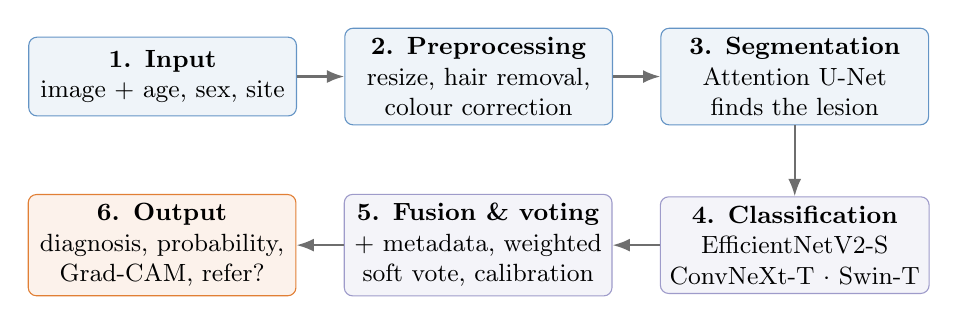
\begin{tikzpicture}[font=\small, node distance=5mm and 6mm,
  st/.style={draw=hcBlue!70,fill=hcBlue!7,rounded corners=3pt,minimum width=34mm,minimum height=10mm,align=center},
  md/.style={draw=hcPurple!70,fill=hcPurple!8,rounded corners=3pt,minimum width=34mm,minimum height=10mm,align=center},
  ot/.style={draw=hcOrange!80,fill=hcOrange!8,rounded corners=3pt,minimum width=34mm,minimum height=10mm,align=center},
  fl/.style={-{Latex[length=2.2mm]},draw=hcGray,thick}]
\node[st] (s1) {\textbf{1. Input}\\image + age, sex, site};
\node[st,right=of s1] (s2) {\textbf{2. Preprocessing}\\resize, hair removal,\\colour correction};
\node[st,right=of s2] (s3) {\textbf{3. Segmentation}\\Attention U-Net\\finds the lesion};
\node[md,below=9mm of s3] (s4) {\textbf{4. Classification}\\EfficientNetV2-S\\ConvNeXt-T $\cdot$ Swin-T};
\node[md,left=of s4] (s5) {\textbf{5. Fusion \& voting}\\+ metadata, weighted\\soft vote, calibration};
\node[ot,left=of s5] (s6) {\textbf{6. Output}\\diagnosis, probability,\\Grad-CAM, refer?};
\draw[fl] (s1)--(s2); \draw[fl] (s2)--(s3); \draw[fl] (s3)--(s4);
\draw[fl] (s4)--(s5); \draw[fl] (s5)--(s6);
\end{tikzpicture}
\caption{System flow at prediction time.}
\label{fig:system}
\end{figure}

\begin{enumerate}
  \item \textbf{Input.} A dermoscopic or smartphone photograph of the
        lesion, with optional age, sex, and body site.
  \item \textbf{Preprocessing.} Resize to $224\times224$ (done). Removing
        hair and ruler marks and correcting colour between cameras are
        planned (next stage).
  \item \textbf{Segmentation (next stage).} An Attention U-Net will
        outline the lesion and crop around it, so that the classifier
        focuses on the lesion, not the surrounding skin.
  \item \textbf{Classification.} Three different networks each predict
        the 8 class probabilities. CNNs capture local texture and colour;
        the Swin transformer captures the global shape and symmetry.
  \item \textbf{Fusion and voting (done).} Temperature scaling makes each
        model's probability trustworthy, and the three outputs are
        averaged (equal weights worked best). Patient metadata will be
        added in the next stage.
  \item \textbf{Output.} The predicted diagnosis, the probability of
        malignancy, and a \emph{refer / monitor} recommendation (done; the
        threshold caught 95.4\% of cancers on the test set). The Grad-CAM
        heatmap is the next stage.
\end{enumerate}

% =====================================================================
\section{Development Flow (How We Build It)}
The project is carried out in seven phases (Fig.~\ref{fig:phases}).
Phases~1--4 are complete: the paper was written, both datasets were
prepared, the three models were trained on an RTX 3060 laptop GPU
(16--17 October 2026), and the measured results were added to the
paper.

\begin{figure}[H]
\centering
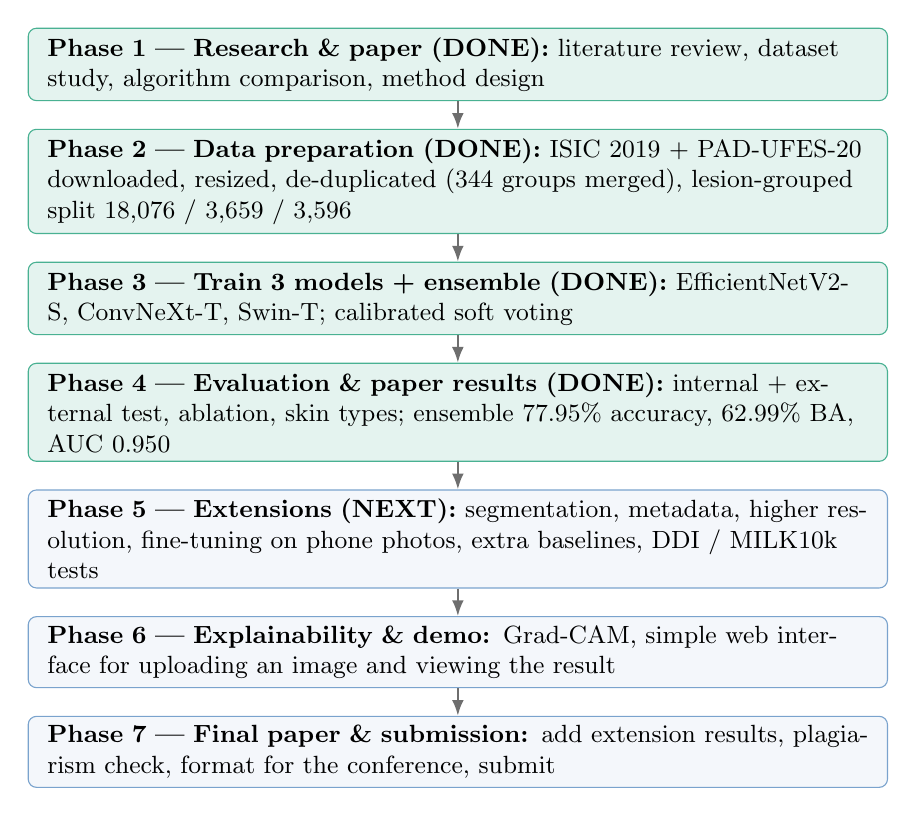
\begin{tikzpicture}[font=\small, node distance=3.5mm,
  done/.style={draw=hcTeal!80,fill=hcTeal!12,rounded corners=3pt,minimum width=0.9\linewidth,minimum height=8.5mm,align=left,text width=0.86\linewidth},
  todo/.style={draw=hcBlue!60,fill=hcBlue!5,rounded corners=3pt,minimum width=0.9\linewidth,minimum height=8.5mm,align=left,text width=0.86\linewidth},
  fl/.style={-{Latex[length=2mm]},draw=hcGray,thick}]
\node[done] (p1) {\textbf{Phase 1 --- Research \& paper (DONE):} literature review, dataset study, algorithm comparison, method design};
\node[done,below=of p1] (p2) {\textbf{Phase 2 --- Data preparation (DONE):} ISIC 2019 + PAD-UFES-20 downloaded, resized, de-duplicated (344 groups merged), lesion-grouped split 18{,}076 / 3{,}659 / 3{,}596};
\node[done,below=of p2] (p3) {\textbf{Phase 3 --- Train 3 models + ensemble (DONE):} EfficientNetV2-S, ConvNeXt-T, Swin-T; calibrated soft voting};
\node[done,below=of p3] (p4) {\textbf{Phase 4 --- Evaluation \& paper results (DONE):} internal + external test, ablation, skin types; ensemble 77.95\% accuracy, 62.99\% BA, AUC 0.950};
\node[todo,below=of p4] (p5) {\textbf{Phase 5 --- Extensions (NEXT):} segmentation, metadata, higher resolution, fine-tuning on phone photos, extra baselines, DDI / MILK10k tests};
\node[todo,below=of p5] (p6) {\textbf{Phase 6 --- Explainability \& demo:} Grad-CAM, simple web interface for uploading an image and viewing the result};
\node[todo,below=of p6] (p7) {\textbf{Phase 7 --- Final paper \& submission:} add extension results, plagiarism check, format for the conference, submit};
\foreach \a/\b in {p1/p2,p2/p3,p3/p4,p4/p5,p5/p6,p6/p7} \draw[fl] (\a)--(\b);
\end{tikzpicture}
\caption{Development phases (green = completed).}
\label{fig:phases}
\end{figure}

\subsection{Phase Details}
{\small
\renewcommand{\arraystretch}{1.25}
\begin{longtable}{@{}L{2.2cm} L{6.6cm} L{3.4cm} L{2.8cm}@{}}
\toprule
\textbf{Phase} & \textbf{Main tasks} & \textbf{Output} & \textbf{Status / time} \\
\midrule
\endhead
1. Research \& paper & Review 40+ studies; study 17 datasets; compare 11 algorithm families; design the method and evaluation protocol & IEEE paper, Datasets and Algorithms reports & Completed \\
2. Data preparation & Download ISIC 2019 (9.8\,GB) and PAD-UFES-20 (3.6\,GB); resize; image-hash de-duplication; map labels to 8 classes; lesion-grouped stratified split & Clean dataset, split files & Completed (about 1 hour incl.\ download) \\
3. Train 3 models + ensemble & EfficientNetV2-S, ConvNeXt-T, Swin-T with focal loss, AdamW, early stopping, TTA; temperature scaling; equal and learned soft voting & Trained models, predictions & Completed (43 + 49 + 36 min on RTX 3060) \\
4. Evaluation \& paper results & Internal and external tests, ablation over model combinations, confusion matrix, ROC, bootstrap CIs, skin-type breakdown; results section, abstract, and conclusion of the paper & Training Results Report, updated paper & Completed \\
5. Extensions & Attention U-Net segmentation, metadata fusion, higher resolution (384\,px), fine-tuning on phone photos, baselines (ResNet-50, DenseNet-121, MobileNetV2, DINOv2), DDI / MILK10k tests & Improved results & Next: about 3--4 weeks \\
6. Explainability \& demo & Grad-CAM for each model; heatmap-in-lesion score; web demo (Streamlit or Flask) & Heatmap figures, demo app & About 2 weeks \\
7. Final paper & Add extension results, plagiarism check, format for the target conference, submit & Submission-ready paper & About 1 week \\
\bottomrule
\end{longtable}
}

% =====================================================================
\section{How the Paper Follows the Project}
We wrote the paper \emph{research-first}: the design and the test rules
were fixed, with published evidence, before we saw any results. After
training, the measured values were added in a new Experimental Results
section (Section~VI), so the paper now contains both the design and the
real results. Table~\ref{tab:map} shows how each section of the paper
corresponds to the project.

{\small
\renewcommand{\arraystretch}{1.25}
\begin{longtable}{@{}L{3.3cm} L{5.4cm} L{3.9cm} L{2.2cm}@{}}
\caption{Paper sections mapped to project work.}\label{tab:map}\\
\toprule
\textbf{Paper section} & \textbf{What it says} & \textbf{Project work} & \textbf{Status} \\
\midrule
\endfirsthead
\toprule
\textbf{Paper section} & \textbf{What it says} & \textbf{Project work} & \textbf{Status} \\
\midrule
\endhead
Abstract \& I.~Introduction & The problem, our contributions, and the measured results & Motivation and objectives & Done (with real numbers) \\
II.~Literature Review & 40+ studies in 7 themes; Table I; six research gaps (G1--G6) & Phase 1 research & Done \\
III.~Datasets & 12 datasets reviewed; ISIC 2019 and PAD-UFES-20 used & Phase 2 & Done \\
IV.~Proposed Methodology & Framework (Fig.~3); implemented part: 3-model ensemble, focal loss, calibration; Algorithm 1; Table III & Phase 3; extensions in Phase 5 & Core done \\
V.~Experimental Design & Leakage-free protocol, metrics, fairness, ablation & Phase 4 & Done \\
VI.~Experimental Results & Training curves, internal/external results, confusion matrix, ROC, ablation, skin types (Figs.~4--7, Tables IV--VII) & Phase 4 & Done \\
VII.~Comparative Analysis & Published results of 11 algorithm families in 4 panels, plus our result & Phases 1 and 4 & Done \\
VIII--IX.~Discussion \& Conclusion & Why the ensemble helps, limitations, accuracy and metrics, future work & Phase 4 & Done \\
\bottomrule
\end{longtable}
}

\subsection{How Each Research Gap Becomes a Project Feature}
{\small
\renewcommand{\arraystretch}{1.25}
\begin{tabularx}{\linewidth}{@{}L{4.6cm} Y@{}}
\toprule
\textbf{Gap found in the literature} & \textbf{What our project did} \\
\midrule
G1: Results are not comparable (random splits, accuracy only) & Removed duplicates, split by lesion, reported balanced accuracy with confidence intervals \\
G2: No testing on outside data & Tested on PAD-UFES-20 (never used in training); MILK10k next \\
G3: Rare cancers (SCC, AK) are neglected & 8-class training with focal loss; per-class recall reported \\
G4: Skin-tone bias & Results per Fitzpatrick type on PAD-UFES-20; DDI next \\
G5: Explanations not evaluated & Grad-CAM with heatmap-in-lesion score (Phase 6) \\
G6: Accurate models are too heavy & All 3 models trained on a 6\,GB laptop GPU in under 1 hour each \\
\bottomrule
\end{tabularx}
}

% =====================================================================
\section{Tools, Team Roles, and Deliverables}
\subsection{Tools and Technology}
\begin{itemize}
  \item \textbf{Language and framework:} Python, PyTorch, \texttt{timm}
        (pre-trained models), \texttt{segmentation\_models\_pytorch}.
  \item \textbf{Explainability:} \texttt{pytorch-grad-cam}.
  \item \textbf{Data:} pandas, OpenCV, \texttt{imagehash} (duplicate
        removal), scikit-learn (GroupKFold, metrics).
  \item \textbf{Hardware:} one NVIDIA GPU; we used an RTX 3060 Laptop
        GPU (6\,GB). Google Colab or Kaggle GPUs also work.
  \item \textbf{Demo:} Streamlit or Flask web interface.
  \item \textbf{Paper:} LaTeX (IEEE template) on Overleaf.
\end{itemize}

\subsection{Suggested Team Roles}
\begin{tabularx}{\linewidth}{@{}L{3.2cm} Y@{}}
\toprule
\textbf{Member} & \textbf{Responsibility} \\
\midrule
Member 1 & Data pipeline: downloads, deduplication, label mapping, splits; segmentation model \\
Member 2 & Classification: baselines, three backbones, metadata fusion, ensemble \\
Member 3 & Evaluation: metrics, external and fairness tests, Grad-CAM, graphs; demo app \\
All + guide & Paper writing, review, and presentation \\
\bottomrule
\end{tabularx}

\subsection{Deliverables}
\begin{enumerate}
  \item IEEE paper with measured results (complete).
  \item Datasets, Algorithms, and Training Results reports (complete).
  \item Source code with training and evaluation scripts
        (\texttt{SkinCancer-training/}, complete).
  \item Trained models, results tables, and graphs (complete).
  \item Web demo showing diagnosis, probability, heatmap, and referral (next).
\end{enumerate}

\subsection{Success Criteria and What We Achieved}
\begin{tabularx}{\linewidth}{@{}L{6.4cm} Y@{}}
\toprule
\textbf{Criterion} & \textbf{Result} \\
\midrule
Ensemble beats every single model & \textbf{Achieved:} 62.99\% BA vs.\ 57.80--60.21\%; 77.95\% vs.\ 73.08--76.89\% accuracy \\
Ensemble beats every pair of models (USP) & \textbf{Achieved:} 3 models $>$ any 2 models on all metrics \\
$\geq$95\% malignant sensitivity at the referral threshold & \textbf{Achieved} internally (95.4\% at 69.9\% specificity); 78.9\% on external phone photos \\
Internal-to-external drop measured and reported & \textbf{Achieved:} accuracy 77.95\% $\rightarrow$ 37.25\%; malignant AUC 0.934 $\rightarrow$ 0.873 \\
Skin-tone gap measured & \textbf{Partly:} types I--II vs.\ III--IV similar; only 11 images of types V--VI (DDI needed) \\
Grad-CAM focuses on the lesion & \textbf{Next stage} \\
\bottomrule
\end{tabularx}

\keybox{\textbf{Summary for the guide:} the project detects skin cancer
from lesion images by combining two CNNs (EfficientNetV2-S, ConvNeXt-T)
and one transformer (Swin-T). The paper was written first as the
evidence-based design (literature review $\rightarrow$ gaps $\rightarrow$
datasets $\rightarrow$ method $\rightarrow$ test rules). The models were
then trained on ISIC 2019 and tested on held-out and external data. The
combined model reached \textbf{77.95\% accuracy, 62.99\% balanced
accuracy, and AUC 0.950}, better than any single model, and these real
results are now in the paper.}

\end{document}
